% Канонический TikZ-рисунок варианта 35. Править только здесь.
\long\def\figStereoV35{%
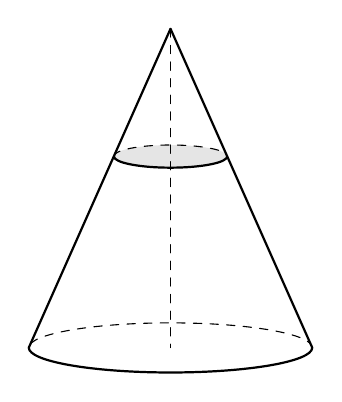
\begin{tikzpicture}[
  scale=0.9,
  line cap=round,
  line join=round
]
  \def\R{2}
  \def\e{0.35}

  \coordinate (S) at (0,4.5);
  \coordinate (L) at (-\R,0);
  \coordinate (R) at ( \R,0);
  \coordinate (O) at (0,0);

  % Центр секущей плоскости
  \coordinate (Q) at (0,2.7);

  % Полупрозрачное сечение
  \fill[black!10]
    (Q) ellipse[x radius=0.8,y radius=0.16];

  % Образующие конуса
  \draw[thick] (S)--(L);
  \draw[thick] (S)--(R);

  % Основание конуса
  \draw[thick]
    (L)
    arc[
      start angle=180,
      end angle=360,
      x radius=\R,
      y radius=\e
    ];

  \draw[dashed]
    (R)
    arc[
      start angle=0,
      end angle=180,
      x radius=\R,
      y radius=\e
    ];

  % Видимая часть линии сечения
  \draw[thick]
    (0.8,2.7)
    arc[
      start angle=0,
      end angle=-180,
      x radius=0.8,
      y radius=0.16
    ];

  % Скрытая часть линии сечения
  \draw[dashed]
    (-0.8,2.7)
    arc[
      start angle=180,
      end angle=0,
      x radius=0.8,
      y radius=0.16
    ];

  % Высота конуса
  \draw[dashed] (S)--(O);
\end{tikzpicture}
}
